

\spis{Obliczenia pól i~objętości – trzy~metody~geometryczne}
{Vazgen Bagdasaryan, Grzegorz~Łukaszewicz}

\wtyt{\hspace*{-5.5cm}Obliczenia pól i~objętości – trzy metody geometryczne}

\waut{Vazgen BAGDASARYAN*, Grzegorz ŁUKASZEWICZ**}
\aafil{Katedra Mechaniki i~Konstrukcji Budowlanych, Szkoła Główna Gospodarstwa
Wiejskiego w~Warszawie

\smallskip
**Wydział Matematyki, Informatyki i~Mechaniki, Uniwersytet Warszawski\bigskip}

\marg{

\includegraphics[width=0.3\textwidth] {Archimedes} 
\\[4pt]
Archimedes z~Syrakuz (ok. 287--212 p.n.e.) -- 
jeden z~najwybitniejszych umysłów matematycznych w~historii. Urodził się i~zmarł w~Syrakuzach. Poza matematyką zajmował się również fizyką i~inżynierią.    
W~swoich czasach wsławił się dzięki wynalazkom mechanicznym – tzw.
\textit{śrubie Archimedesa} do pompowania wody, dźwigni,
planetarium~(bardzo dokładnie odtwarzającym ruchy ciał niebieskich) oraz maszynom wojennym, które przerażały rzymskich żołnierzy podczas oblężenia Syrakuz (oblężenie to przyniosło śmierć Archimedesowi).
Niestety tylko niektóre dzieła Archimedesa przetrwały do naszych czasów.
Należy do nich ważny traktat zatytułowany ,,Metoda'',
który został ponownie odkryty dopiero w~1906 roku, w~Konstantynopolu,
praktycznie przez przypadek -- w~palimpseście~powstałym w~roku 1229. W~tym traktacie Archimedes szczegółowo opisał
swoją {\it metodę dźwigni}. Historia wspomnianego palimpsestu (zawierającego także inne
traktaty Archimedesa) i~metody użyte do jego prawidłowego odczytania są
przedstawione w~bardzo ciekawej książce Reviela Netza i~Williama Noela [4].  }

\vspace*{-1cm}
\begin{flushright}
% \begin{minipage}{6cm}
{\it Największe pomysły cechuje prostota}\\
William Golding
% \end{minipage}
\end{flushright}

\vspace*{-.2cm}
Obliczanie pól figur płaskich i~objętości brył, nawet w~prostych przypadkach,
bywa czasem dość kłopotliwe, np. wtedy, gdy łatwo jest napisać całkę wyrażającą
pole figury, ale samo obliczenie tej całki jest niebanalne. Zagadnieniem {\it
metod obliczania} pól i~objętości zajmowało się wielu wybitnych matematyków,
począwszy od czasów starożytnych aż po nam współczesne.    

W~tym artykule przedstawiamy trzy geometryczne  podejścia do wyznaczania pól i~objętości opracowane w~różnych epokach: podejście Archimedesa (III w. p.n.e.), Cavalieriego (XVII w.) oraz Mamikona Mnatsakaniana (XX w.).

{\bf \color{magenta}Metoda I~– podejście Archimedesa.}
Archimedes uważany jest za jednego z~twórców statyki i~hydrostatyki. Obliczył on środki ciężkości wielu ważnych figur geometrycznych i~brył, między innymi trójkąta, trapezu, dowolnego wycinka paraboli i~segmentu paraboloidy obrotowej.  
Swoje wyniki dotyczące statyki zawarł w~dziełach {\it O~równowadze płaszczyzn} i~{\it Kwadratura paraboli}. 

{\it Prawo dźwigni}, sformułowane przez Archimedesa, jest jednym z~praw równowagi, należy do statyki i~mówi, że:  

{\it Wielkości są w~równowadze w~odległościach odwrotnie proporcjonalnych do ich wag.}

Jeżeli po obu stronach dźwigni umieścimy masy, odpowiednio, $m$ i~$m'$, a~odległości ich środków ciężkości od punktu podparcia dźwigni, odpowiednio, $d_S$ i~$d_{S'}$, są do siebie w~stosunku odwrotnie proporcjonalnym do stosunków tych mas:
\begin{eqnarray}
\frac{d_S}{d_{S'}}=\frac{m'}{m},
\end{eqnarray}
to dźwignia pozostaje w~równowadze statycznej.

Jeśli przyjmiemy, że obie masy mają tę samą stałą gęstość, to $m'/m=V'/V$, gdzie $V'$ i~$V$ są objętościami mas, odpowiednio, $m'$ i~$m$. 
Zatem 
\begin{eqnarray}
\frac{d_S}{d_{S'}}=\frac{V'}{V}.
\end{eqnarray}
Gdy rozważamy  wyidealizowany problem dwuwymiarowy, objętości $V'$ i~$V$ zamieniamy na pola $A'$ i~$A$ dwóch figur płaskich. 

Powyższą zasadę można wykorzystać w~celu wyznaczania pól i~objętości
w~następujący sposób (por. [2]). Przypuśćmy, że $R$ i~$S$ to dwa
obszary leżące wzdłuż tego samego odcinka osi poziomej (rys. 1). Mając dane pole
$A(S)$ oraz środek ciężkości $c_S$ obszaru $S$, pytamy o~pole $A(R)$ obszaru $R$.

\marg[-60]{
\begin{tikzpicture}[x=.15cm,y=.15cm]
\tikzset{font=\scriptsize}
%%% parameters
\def\dmin{1} % domain minimum
\def\dmax{18} % domain maximum
\def\Sheight{5} % heiggt of S
\def\xo{-3} % position of point O
\def\Slw{.4} % line width for S 
\def\Scol{black} % color of S
\def\Rcol{black} % color of R
\def\Rlw{.4} % line width for R 
\def\alw{.4} % line width for axis
\def\xmin{-26} % beginning of axis
\def\xmax{18.5} % end of axis
\def\ts{1.5} % triangle size
\def\k{22}
\def\x{10}
\def\xs{14}
\def\ps{.5} % point size in mm
\def\auxha{12} % height of auciliary line 1
\def\auxhb{10} % level of auciliary line 
\def\auxhc{8} % level of auciliary line 

%%% computed
\pgfmathsetmacro{\leftSy}{\dmin^(1/2)}
\pgfmathsetmacro{\rightSy}{\dmax^(1/2)}

%%% drawing

%% S
\draw[color=\Scol, 
			samples=100, 
			line width=\Slw, 
			domain=\dmin:\dmax] 
	(\dmin,-\leftSy-\Sheight)--(\dmin,\leftSy+\Sheight)
	(\dmax,-\rightSy-\Sheight)--(\dmax,\rightSy+\Sheight)
	plot (\x,{\x^(1/2)+\Sheight}) 
	plot (\x,{-\x^(1/2)-\Sheight});

%% R
\draw[color=\Rcol, 
			samples=100, 
			line width=\Rlw, 
			domain=\dmin:\dmax] 
	(\dmin,-\leftSy-\Sheight)--(\dmin,\leftSy+\Sheight)
	(\dmax,-\rightSy-\Sheight)--(\dmax,\rightSy+\Sheight)
	plot (\x,{(\x-\xo)*(\x^(1/2)+\Sheight)/\k}) 
	plot (\x,{(\x-\xo)*(-\x^(1/2)-\Sheight)/\k});

%% axis
\draw[line width=\alw] 
	(\xmin,0)--(\xmax,0);

%%% triangle
\filldraw[black, shift=({\xo,-\ts})] (90:\ts)--(210:\ts)--(330:\ts);

%%% points etc.
\node (P) at (\xo-\k,0) {};
\node (cS) at (\xo+\xs,0) {};
\node (O) at (\xo,0) {};
\pgfmathsetmacro{\midSy}{(\xo+\x)^(1/2)}

\filldraw[black] (P) circle (\ps);
\filldraw[black] (cS) circle (\ps);
\draw[line width=\alw] 
	(\xo+\x,-\midSy-\Sheight)--(\xo+\x,\midSy+\Sheight);

%%% auxiliary lines
\draw[ dashed, line width=\alw] (P)--++(0,\auxha);
\draw[ dashed, line width=\alw] (cS)--++(0,\auxha);
\draw[ dashed, line width=\alw] (\xo,0)--++(0,\auxha);
\draw[ dashed, line width=\alw] (\xo+\x,0)--++(0,\auxha);

\draw[Stealth-Stealth, line width=\alw/2, shift=({0,\auxhc})]%, gray] 
	(\xo-\k,0)--(\xo,0)
	node [midway,above] {$k$};
\draw[Stealth-Stealth, line width=\alw/2, shift=({0,\auxhc})]%, gray] 
	(\xo+\x,0)--(\xo,0)
	node [pos=.6,below left] {$x$};
\draw[Stealth-Stealth, line width=\alw/2, shift=({0,\auxhb})]%, gray] 
	(\xo+\xs,0)--(\xo,0)
	node [midway,above] {$x_S$};
\draw[Stealth-Stealth, line width=\alw/2, shift=({-.5,0})]%, gray] 
	(\xo+\x,-\midSy-\Sheight)--(\xo+\x,\midSy+\Sheight)
	node [pos=.1,above left, shift=({.4,0})] {$\quad l'$};
\pgfmathsetmacro{\nh}{(\midSy+\Sheight)*\x/\k}
\draw[Stealth-Stealth, line width=\alw/2, shift=({.5,0})]%, gray] 
	(\xo+\x,-\nh)--(\xo+\x,\nh)
	node [pos=.05,above right] {$l$};

%%% labelling
\node[below=.5 of P.center] {$P$};
\node[above left=.2 and .2 of O.center] {$O$};
\node at (\dmin+1,-5) {$S$};
\node at (\dmax-1.2,-5) {$R$};
\node[below=.5 of cS.center] {$c_S$};
\end{tikzpicture}
\\[4pt]
{Rys. 1} %[Na tym rysunku jest błąd. Powinno być spełnione $x\cdot l'/l=\textrm{const}$, a~nie jest -- przyp. ŁR]
}%
\hspace*{1.5cm}
\begin{minipage}{11cm}\raggedright
Obszary $R$ i~$S$ są wypełnione liniami pionowymi, odpowiednio, $l$ i~$l'$ tak, że każda linia $l$ (odp. $l'$) jest zawarta w~obszarze $R$ (odp. $S$), a~każdy punkt obszaru $R$ (odp. $S$) należy do dokładnie jednej linii $l$ (odp. $l'$).

Przypuśćmy, że istnieje taka stała $k$, że dla każdej pionowej linii w~odległości $x$ od punktu $O$, przecinającej obszary $R$ i~$S$ w~odcinkach o~długościach $l$ i~$l',$ odpowiednio, spełniona jest relacja
\begin{equation*}
\frac{k}{x}=\frac{l'}{l}\,.
\end{equation*}
Wówczas z~prawa dźwigni wynika, że odcinek $l$ umieszczony w~punkcie~$P$,
w~odległości $k$ od punktu podparcia $O$, równoważy odcinek $l'$ w~miejscu,
w~którym się znajduje. 
\end{minipage}\goodbreak

Zatem jeśli obszar $R$ zostanie umieszczony tak, aby
jego środek ciężkości znalazł się w~punkcie $P$, to zrównoważy on obszar $S$
w~miejscu, w~którym się znajduje, co prowadzi do równania 
\begin{equation*} 
\frac{k}{x_S}=\frac{A(S)}{A(R)}, 
\end{equation*}
gdzie $x_S$ to odległość środka ciężkości $c_S$ obszaru $S$ od punktu $O$. Znając $A(S)$, $x_S$ oraz $k$, z~powyższego równania obliczamy szukaną wielkość $A(R)$.

{\bf Przykład 1.} {\it Obliczenie pola pod parabolą}. Weźmy za $R$
obszar ograniczony przez parabolę $y=x^2$, oś $OX$ oraz prostą $x=1$. Niech $S$
będzie trójkątem o~wierzchołkach w~punktach $(0,0)$, $(1,0)$, $(1,1)$, którego
pole powierzchni wynosi $A(S)=\frac{1}{2}$, a~środek ciężkości ma pierwszą
współrzędną $x_{S}=\frac{2}{3}$. 
\marg{
\begin{tikzpicture}[scale=2]
\draw[-latex](0,-.3)--(0,1.25);
\draw[-latex](-1.25,0)--(1.25,0);
\draw[blue,fill=blue!10](0,0)--(1,1)--(1,0)--cycle;
\draw[orange]	
	plot[samples=20,domain=0:1]
	(\x, {\x*\x});
\begin{scope}
\pgfsetfillpattern{dots}{blue}
\draw[magenta,pattern={Lines[
                  distance=2mm,
                  angle=90,
                  line width=0.07mm
                 ]}%north west lines
, pattern color=magenta] (0,0) parabola (1,1) -- (1,0) -- cycle;
\end{scope}
\node[below right] at(0,0){$(0,0)$};
\node[above] at(1.2,0){$x$};
\node[left] at(0,1.2){$x$};
\node at(.85,.4){$y{=}x^{2}$};
\node at(.8,.1){$R$};
\node at(.4,.3){$S$};
\node at(.4,.6){$y{=}x$};
\node[below] at(1,0){$(1,0)$};
\node[above] at(1,1){$(1,1)$};
\node[below] at(-1,0){$(-1,0)$};
\node[above] at(-1,0){$P$};
\draw[fill](-1,0) circle(.02);
\end{tikzpicture}\\[4pt]
{Rys. 2} %[zamiast poziomych linii wstawić pionowe, w~miejscach pomiędzy obecnymi pionowymi-- przyp. ŁR]
}

Mamy $l=x^2$, a~$l'=x$, zatem możemy przyjąć $k=1$ i~otrzymujemy $1 \cdot x^2=x \cdot x$. Oznacza to (przy założeniu, że oś $OX$ jest dźwignią podpartą w~punkcie $(0,0)$), że gdybyśmy przesunęli obszar $R$ pod parabolą tak, aby jego środek ciężkości znalazł się w~punkcie $P$ o~współrzędnych $(-1,0)$, to zrównoważyłby on trójkąt w~miejscu, w~którym się znajduje. Otrzymujemy zatem:
\begin{equation*}
A(R) = A(S) \cdot x_S = \frac{1}{2} \cdot \frac{2}{3} = \frac{1}{3}.
\end{equation*}
W~celu wykorzystania tej metody do wyznaczenia objętości brył należy zastąpić długości odcinków polami powierzchni przekrojów poprzecznych. Jako ilustrację przytoczymy jeden z~najważniejszych wyników otrzymanych przez Archimedesa.

{\bf Przykład 2.} [2] {\it Obliczenie objętości kuli}. 
\marg{\vspace*{0cm}
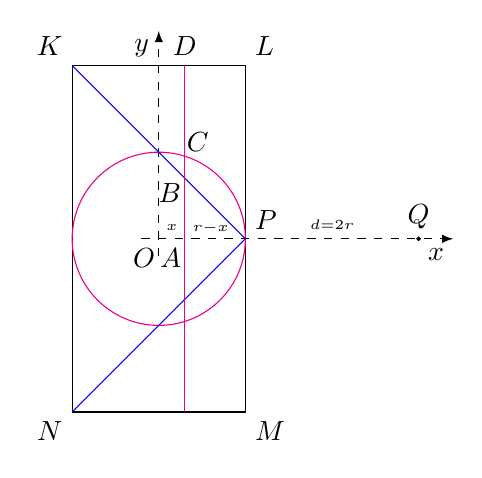
\begin{tikzpicture}[scale=1.1]
  \draw(0,0) rectangle(2,4);
  \draw[dashed,-latex](.8,2)--(4.4,2);
  \draw[dashed,-latex](1,1.8)--(1,4.4);
  \draw[fill](4,2) circle(.02);
  \node[above] at(4,2){$Q$};
  \draw[magenta](1,2) circle(1);
  \draw[blue](0,4)--(2,2)--(0,0);
  \draw[very thin,magenta](1.3,0)--(1.3,4);
  \node[below left] at (1.07,2){$O$};
  \node[below left] at (1.37,2){$A$};
  \node[below left] at (1.37,2.75){$B$};
  \node[above] at (1.45,2.9){$C$};
  \node[above] at (1.15,1.98){\tiny$x$};
  \node[above] at (1.6,1.95){\tiny$r{-}x$};
  \node[above] at (3,2){\tiny$d{=}2r$};
  \node[left] at(1,4.2){$y$};
  \node[below] at(4.2,2){$x$};
  \node[below left] at(0,0){$N$};
  \node[above left] at(0,4){$K$};
  \node[above right] at(2,4){$L$};
  \node[above right] at(2,2){$P$};
  \node[below right] at(2,0){$M$};
  \node[above] at(1.3,4){$D$};
  \end{tikzpicture}\\[4pt]
{Rys. 3}
}
Konstrukcję rozpoczynamy od narysowania okręgu $x^2+y^2=r^2$ przecinającego oś $OX$ w~punkcie 
$P=(r,0)$. Następnie rysujemy prostokąt $KLMN$, którego środek ciężkości
umiejscowiony jest w~środku układu współrzędnych. Jego podstawa ma długość
$d=2r$, a~jego wysokość jest równa $h=2d$. Rysujemy również trójkąt $KNP$. Przez
obrót tych figur wokół osi $OX$ otrzymujemy bryły: kulę $S$, stożek $C$ oraz
walec~$Z$. Zauważmy, że otrzymane bryły zbudowane są z~dysków prostopadłych do osi~$OX$. Dla przykładu, przekrój płaszczyzną prostopadłą do osi $OX,$ przechodzącą przez punkt $A=(x,0)$ przecina kulę – tworząc koło $S_x$ o~promieniu ${AC=y=\sqrt{r^2-x^2}}$, stożek – tworząc koło $C_x$ o~promieniu $AB=r-x$ oraz walec – tworząc koło $Z_x$ o~promieniu $AD=d=2r$. Przeprowadźmy rachunki:
\begin{align*}
d \cdot [A(S_x)+A(C_x)] &= \pi d \cdot [y^2+(r-x)^2] \\&= \pi d \cdot [(r^2-x^2)+(r^2-2rx+x^2)] \\&= 
\pi d \cdot (2r^2-2rx) \\&= \pi d^2 \cdot (r-x) \\&= (r-x) \cdot A(Z_x).
\end{align*} 
Mamy zatem
\begin{equation*}
d \cdot [A(S_x)+A(C_x)] = (r-x) \cdot A(Z_x),
\end{equation*}
co oznacza, że jeśli przyjmiemy, że oś $OX$ jest dźwignią z~podparciem w~punkcie~$P,$ oraz umieścimy koła $S_x$ i~$C_x$ w~punkcie $Q=(3r,0),$ to razem zrównoważą koło $Z_x$ w~miejscu, w~którym się znajduje. To prowadzi do wniosku, że jeśli kulę $S$ oraz stożek $C$ umieścimy tak, aby ich środki ciężkości znalazły się w~punkcie~$Q$, to razem zrównoważą one walec $Z$ w~miejscu, w~którym się znajduje. Zatem zasada dźwigni implikuje relację:
\begin{equation*}
2r \cdot [V(S)+V(C)] = r \cdot V(Z).
\end{equation*}
Podstawiając znane objętości $V(C)=\frac{1}{3} \pi d^3$ oraz $V(Z) = \pi d^3$, obliczamy objętość kuli o~promieniu $r$:
\begin{equation*}
V(S) = \frac{1}{6} \pi d^3 = \frac{4}{3} \pi r^3.
\end{equation*}
\marg[-158]{


\includegraphics[width=0.3\textwidth]
{Cavalieri} \\[4pt]
Bonaventura Francesco Cavalieri (1598--1647).
Włoski matematyk i~astronom. Studiował na uniwersytetach w~Pizie i~w~Bolonii. Był uczniem Galileusza. Zajmował się głównie geometrią.
Jako pierwszy zaczął stosować metody nieskończenie małych elementów do obliczania pól powierzchni i~objętości
}{\bf \color{magenta} Metoda II – podejście Cavalieriego.}
Bonaventura Cavalieri spopularyzował swoją metodę w~dwóch pracach, {\it Geometria indivisibilibus} z~1635 roku oraz {\it Exercitationes geometricae sex} z~1647 roku. 
Opiera się ona na zasadzie znanej jako     twierdzenie Cavalieriego.
\goodbreak

{\bf Twierdzenie Cavalieriego.} [2] {\it Jeśli dwie bryły mają tę własność, że ich przekroje wszystkimi płaszczyznami równoległymi do jednej, z~góry ustalonej płaszczyzny mają te same pola, to te bryły mają równe objętości.
Jeśli przekroje na równych wysokościach są w~stałym stosunku, to objętości tych brył również są w~tym stosunku.}

\smallskip
{\bf Przykład 3.} {\it Obliczenie objętości stożka.}  
Zauważmy najpierw, że  możemy łatwo wyznaczyć pola powierzchni przekrojów stożka oraz ostrosłupa na dowolnej wysokości. Mamy (patrz rys. 4)
\begin{equation*}
A(C_x)=\frac{\pi r^2 x^2}{h^2} \quad \textrm{oraz} \quad A(P_x)=\frac{x^2}{h^2}.
\end{equation*}

\marg{

%\begin{figure}[h] 
%  \centering
  
\includegraphics[scale=0.4]{przekroje Cavalieri.png}%
  \raise60pt\llap{$P_{x}$\kern28pt}%
  \raise61pt\llap{$C_{x}$\kern76.5pt}%
  \raise67.5pt\llap{$x$\kern117pt}%
  \raise35pt\llap{$P$\kern-2pt}%
  \raise35pt\llap{$C$\kern74pt}%
  \raise42pt\llap{$h$\kern128pt}%
  \raise8pt\llap{$r$\kern86pt}%
  \raise3pt\llap{1\kern5pt}%
  \raise4pt\llap{1\kern28pt}%
    
{Rys. 4}
%\end{figure}
}Ponieważ stosunek tych pól na dowolnej wysokości jest stały i~nie zależy od $x$, 
\begin{equation*}
\frac{A(C_x)}{A(P_x)}=\pi r^2,
\end{equation*}
więc, na podstawie twierdzenia Cavalieriego, stosunek objętości brył jest taki sam. Znając objętość ostrosłupa ($V(P)=\frac{1}{3}\cdot 1 \cdot h$), łatwo teraz wyznaczamy objętość stożka:
\marg{Więcej przykładów zastosowania zasady Cavalieriego można znaleźć
w~artykule Jarosława Górnickiego
z~\href{https://www.deltami.edu.pl/2012/01/zasada-cavalieriego/}{$\Delta^{1}\sb{12}$.}}
\begin{equation*}
\frac{V(C)}{V(P)}=\pi r^2 \Rightarrow V(C)=\pi r^2 V(P) = \frac{1}{3} \pi r^2 h.
\end{equation*}
{\bf \color{magenta} Metoda III – podejście Mamikona.}
\marg{\vspace*{1.5cm}



\includegraphics[width=5cm]{m-a}
\\[4pt]
Mamikon Mnatsakanian (po lewej), Tom~M.~Apostol (po prawej)

\bigskip
Mamikon Mnatsakanian (1942--2021).
Ormiański fizyk, który na metodę „{\it całkowania wizualnego}” wpadł w~trakcie
studiów. Pomysł ten jednak przez wiele lat nie został zauważony i~doceniony.
Dopiero w~trakcie pobytu Mamikona w~USA prof. Tom M.
Apostol dostrzegł w~jego metodzie potencjał i~wspólnie zaczęli się nią zajmować i~rozwijać. 

\smallskip
{\it ,,Jako nauczyciel rachunku różniczkowego z~ponad 50-letnim stażem i~autor kilku podręczników na ten temat byłem zdumiony, gdy dowiedziałem się, że wiele standardowych problemów w~rachunku różniczkowym można łatwo rozwiązać za pomocą innowacyjnego podejścia wizualnego, które nie korzysta ze wzorów''.} -- Tom M. Apostol

}
Przytoczymy tu tylko jeden z~całej bogatej kolekcji pomysłów Mamikona
Mnatsakaniana, odsyłając zainteresowanego Czytelnika do dalszej lektury [1]. 
Przedstawiony tu pomysł ma źródło w~prostej obserwacji. Zastanówmy się, ile wynosi pole powierzchni pierścienia zawartego pomiędzy dwoma okręgami o~wspólnym środku, w~którym długość cięciwy większego okręgu, stycznej zewnętrznie do mniejszego okręgu, wynosi $a$? 
\medskip

\hbox to\textwidth{\kern.67cm\scriptsize\vbox{\hsize5.5cm
 
   
\includegraphics[scale=0.27]{Mamikon - motywacja.png}%
    \raise59pt\llap{$a$\kern112pt}%
    \raise59pt\llap{$a/2$\kern17pt}%
    \raise45pt\llap{$r$\kern38pt}%
    \raise37pt\llap{$R$\kern18pt}%
         \llap{Rys. 5\kern5.2cm} 
        

}\kern1cm\vbox{\hsize5.5cm  
\includegraphics[scale=0.27]{Mamikon - miotla.png}
    \raise61pt\llap{$L$\kern100pt}%
    \raise39pt\llap{$L$\kern13pt}%
    \llap{Rys. 6\kern5cm}}}

Standardowy rachunek jest prosty, odpowiedź to (przy oznaczeniach z~rys. 5):
\begin{equation*}
\pi R^2 - \pi r^2 = \pi (R^2-r^2)=\pi \biggl(\frac{a}{2}\biggr)^2,
\end{equation*} %
gdzie w~ostatniej równości skorzystaliśmy z~twierdzenia
Pitagorasa. Pole to nie zależy zatem od promieni okręgów, a~jedynie od długości cięciwy stycznej do
wewnętrznego okręgu. Obserwacja ta stała się przyczynkiem do rozważań na temat
wyznaczenia tego pola w~inny sposób. 

Wyobraźmy sobie, że połowa wspomnianej cięciwy jest wektorem $\vec L$ o~długości $L=\frac{a}{2}$, który obracamy wokół mniejszego okręgu tak, że w~każdym miejscu jest on styczny do tego okręgu. 
Wykonując pełny obrót, zakreślimy cały interesujący nas obszar. Mamikon
spostrzegł, że po zaczepieniu wszystkich tych wektorów w~jednym punkcie
otrzymamy koło o~promieniu równym długości obracanego wektora i~polu równym $\pi
L^2$~(rys. 6). Pole to jest oczywiście równe polu rozważanego pierścienia (zauważmy, że
to rozumowanie nie wymaga użycia twierdzenia Pitagorasa). 

% \marg{\
% \includegraphics[width=0.25\textwidth]
% {Mamikon - Pitagoras} \hspace{0.2cm}
% 
% {Rys. 7} \\
% 
% Spostrzeżenie Mamikona i~twierdzenie Pitagorasa. 
% Z jednej strony pole błękitnego pierścienia jest równe $\pi R^2-\pi r^2$. Z~drugiej strony, korzystając z~obserwacji Mamikona, pole to wynosi $\pi L^2$. Zatem $R^2 - r^2= L^2$ lub $R^2= L^2+ r^2$, co jest treścią twierdzenia Pitagorasa, a~powyższe rozumowanie jeszcze innym jego dowodem.
% 
% \hspace{0.2cm}
% }

Powyższą sytuację możemy zinterpretować w~ramach mechaniki Newtona jako
szczególny przypadek  ogólniejszego twierdzenia mówiącego o~tym, że hodograf
prędkości ruchu po elipsie w~polu Newtonowskim z~centrum w~jednym z~jej ognisk
jest okręgiem o~promieniu $r=\frac{v_P+v_A}{2}$, gdzie $v_P$ i~$v_A$ są
prędkościami, odpowiednio, w~peryhelium i~aphelium elipsy (por. artykuł
\textit{William Rowan Hamilton i~hodograf} z~\href{https://www.deltami.edu.pl/2024/09/william-rowan-hamilton-i-hodograf/}{$\Delta^{9}\sb{24}$}).

Mamikon uogólnił swoje spostrzeżenie, formułując następujące twierdzenie,
dotyczące krzywych niekoniecznie zamkniętych, do których wektory styczne nie muszą mieć tej samej długości w~każdym punkcie krzywej.

{\bf Twierdzenie Mamikona} (postać ogólna).
\marg{Twierdzenie Mamikona pozostaje prawdziwe również dla krzywych
w~przestrzeni trójwymiarowej.}
{\it Pole zakreślenia stycznego dla dowolnej gładkiej krzywej jest
równe polu jego pęku stycznego.}

Przez ,,zakreślenie styczne'' rozumiemy obszar złożony z~rozłącznych odcinków stycznych
do krzywej, a~przez ,,pęk styczny'' -- zbiór powstały przez takie przesunięcie
owych odcinków, by pozostały one rozłączne i~pokryły się punkty ich styczności do krzywej.
Na rysunku 6 widzimy przykład zakreślenia stycznego do wewnętrznego okręgu po lewej
stronie i~jego pęk styczny po prawej stronie rysunku. Wspomniany wyżej hodograf
prędkości dla ruchu po elipsie w~polu Newtonowskim jest następnym przykładem
\marg{
\begin{center}

\includegraphics[width=5cm]{hodograf.png}
\end{center}
Rys.~7 %[Ten rysunek być może łatwiej odrysować na podstawie rysunku z~tekstu Łukaszewicza o~hodografie (9/2024))]
}
pęku stycznego, także będącego okręgiem~(rys. 7). Tym razem zakreślenie styczne składa
się z~wektorów o~różnej długości. 

W~celu zilustrowania powyższego twierdzenia pokażemy dwa przykłady dotyczące krzywych na płaszczyźnie.  


{\bf Przykład 4.}
{\it Wyznaczenie pola powierzchni pomiędzy wykresem funkcji eksponencjalnej
a~osią odciętych w~granicach od minus nieskończoności do ustalonego $x$}. W~celu
zrozumienia rozwiązania ważne jest zauważenie, że dla funkcji
$y=e^{\frac{x}{b}}$ odcinek łączący dowolny punkt $(x,0)$ na osi odciętych z~miejscem
przecięcia tej osi ze styczną do wykresu funkcji w~{punkcie
$(x,e^{\frac{x}{b}})$} ma stałą długość równą $b$ (patrz rys. 8).
\marg{


\includegraphics[width=4.7cm]
{Mamikon - ekspotencjalna}%
\raise60pt\llap{$y\!=\!e^{x/b}$\kern-20pt}%
\lower8pt\llap{$b$\kern100pt}%
\lower8pt\llap{$b$\kern22pt}%
\lower8pt\llap{$b$\kern67pt}%
\lower8pt\llap{$x$\kern7pt}%
\\[4pt]
{Rys. 8}
\hspace{0.2cm}

\hspace{0.2cm}
}\marg{

\hspace*{3mm}
\includegraphics[width=4.5cm]
{Mamikon - parabola2}%
\raise70pt\llap{$x/2$\kern55pt}%
\raise163pt\llap{$x/2$\kern60pt}%
\raise193pt\llap{$S$\kern60pt}%
\raise163pt\llap{$0$\kern120pt}%
\raise70pt\llap{$x$\kern12pt}%
\raise163pt\llap{$x$\kern12pt}%
\raise180pt\llap{$T$\kern22pt}%
\raise238pt\llap{$x^{2}$\kern7pt}%
\raise238pt\llap{(a)\kern125pt}%
\raise138pt\llap{(b)\kern125pt}%
\raise76.5pt\llap{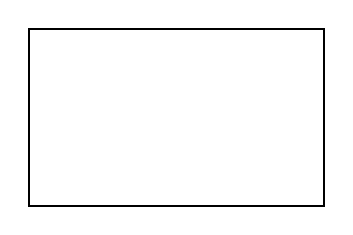
\begin{tikzpicture}[line width=.75pt]
\draw  (0,0) rectangle (3.75,2.25);
\end{tikzpicture}\kern13.4pt}
{Rys. 9}
\hspace{0.2cm}

\hspace{0.2cm}
}


Zauważmy, że przenosząc wszystkie odcinki styczne do miejsca przecięcia stycznej do krzywej w~punkcie 
$(x, e^\frac{x}{b})$ z~osią $OX$, zapełniamy trójkąt prostokątny
o~przyprostokątnych~długości $b$ i~$e^{\frac{x}{b}}$. 
Trójkąt ten wypełnia zatem połowę pola powierzchni pod
wykresem, które wobec tego musi być równe
$2 \cdot \frac{1}{2} b e^\frac{x}{b}=b e^\frac{x}{b}$. 

{\bf Przykład 5.}
{\it Wyznaczenie pola powierzchni pomiędzy wykresem funkcji $x^n$ a~osią odciętych w~granicach od zera do ustalonego $x$}. Dla ustalenia uwagi przyjmiemy $n=2$ (dla innych potęg rozumowanie jest analogiczne).

%\begin{figure}[h] 
%  \centering
%    \includegraphics[scale=0.5]{Mamikon - %parabola.png}
%\end{figure}

Zauważmy, że figura, której pola szukamy, zawarta jest w~prostokącie o~bokach równych $x$ i~$x^2$, zatem na pewno jest to część pola powierzchni tego prostokąta równego $P = x^3$. Archimedes jako pierwszy obliczył,
przy pomocy metody dźwigni, że pole to wynosi 
$\frac{1}{3}P$ (patrz przykład 1). Poniżej pokażemy, jak można uzyskać ten wynik w~dość prosty sposób, oparty na elementarnym podejściu geometrycznym. 
To, co będzie nam potrzebne, to fakt, że styczna do paraboli w~punkcie o~odciętej
$x$ przecina oś $OX$ w~punkcie o~odciętej $\frac{x}{2}$ ($=x-\frac{x^2}{2x}$).   Styczna ta dzieli naszą figurę na dwie części, na rysunku oznaczone przez $S$ oraz $T$. Figura $S$ powstaje przez narysowanie wszystkich odcinków stycznych do paraboli i~kończących się na osi $OX$. 


\marg{Metodę Mamikona
można również odnaleźć w~artykule \textit{W~którą stronę
jechał rower?}
z~\href{https://www.deltami.edu.pl/2022/08/w-ktora-strone-jechal-rower/}{$\Delta^8\sb{22}$}.}
\marg{\vspace*{1.5cm}
\textbf{Literatura}

[1] T. M. Apostol, M. A. Mnatsakanian, {\it New Horizones in Geometry}, The Mathematical Association of America, 2012.

[2] C. H. Edwards, {\it The Historical Development of the Calculus}, Springer-Verlag, NewYork, 1979.

[3] P. Lynch, {\it Mamikon’s Visual Calculus and the Hodograph}, Mathematics
Today, April 2022, 212-214.

[4] R. Netz, W. Noel, {\it Kodeks Archimedesa}, Magnum, 2002.

}%
Przedłużmy teraz odcinki tworzące obszar $S$ do przecięcia z~osią $OY$
(rys. 9b). 
Z~wcześniejszej obserwacji dotyczącej ich punktu przecięcia z~osią $OX$ wynika,
że w~ten sposób każdy z~nich został przeskalowany przez $t=2$.
Z~twierdzenia Mamikona i~twierdzenia o~jednokładności wynika, że
zakreskowany obszar ma pole powierzchni równe $t^2A(S)=4A(S)$.
Dlatego obszar pod osią
$OX$ ma powierzchnię równą $3A(S)$. Jednocześnie obszar ten
jest przystający do obszaru $T$. 
Zatem $A(T)=3A(S)$ oraz $4A(T) = P$, skąd otrzymujemy ${A(T\cup S) = \frac{1}{3}P=\frac{1}{3}x^3}$. 

Wszystkie powyższe obliczenia można łatwo otrzymać, korzystając z~rachunku
całkowego w~ujednolicony sposób, dość mechanicznie i~prawie bez żadnego nakładu
myślowego. Pokazuje to siłę rachunku całkowego, w~którym rozumowanie jest ukryte
w~,,czarnej skrzynce'', a~do nas należy włożenie danych, ,,pokręcenie korbką''
i~wyjęcie gotowego wyniku. Jednak ten brak naoczności Leibnizowskiej wersji
rachunku różniczkowego i~całkowego był jedną z~przyczyn, dla których Isaac
Newton napisał {\it Principia} w~języku geometrii starożytnych i~geometrycznej
wersji tegoż rachunku. Dzisiaj, w~świecie mechanizacji myślenia, w~którym palec
(od naciskania klawiszy lub ekranu) boli nas często bardziej niż głowa, przypomnienie
wartości piękna, prostoty i~głębi rozumowań geometrycznych staje się coraz
cenniejsze, nie tylko w~dydaktyce matematyki i~fizyki.  
